\documentclass[1p]{elsarticle_modified}
%\bibliographystyle{elsarticle-num}

%\usepackage[colorlinks]{hyperref}
%\usepackage{abbrmath_seonhwa} %\Abb, \Ascr, \Acal ,\Abf, \Afrak
\usepackage{amsfonts}
\usepackage{amssymb}
\usepackage{amsmath}
\usepackage{amsthm}
\usepackage{scalefnt}
\usepackage{amsbsy}
\usepackage{kotex}
\usepackage{caption}
\usepackage{subfig}
\usepackage{color}
\usepackage{graphicx}
\usepackage{xcolor} %% white, black, red, green, blue, cyan, magenta, yellow
\usepackage{float}
\usepackage{setspace}
\usepackage{hyperref}

\usepackage{tikz}
\usetikzlibrary{arrows}

\usepackage{multirow}
\usepackage{array} % fixed length table
\usepackage{hhline}

%%%%%%%%%%%%%%%%%%%%%
\makeatletter
\renewcommand*\env@matrix[1][\arraystretch]{%
	\edef\arraystretch{#1}%
	\hskip -\arraycolsep
	\let\@ifnextchar\new@ifnextchar
	\array{*\c@MaxMatrixCols c}}
\makeatother %https://tex.stackexchange.com/questions/14071/how-can-i-increase-the-line-spacing-in-a-matrix
%%%%%%%%%%%%%%%

\usepackage[normalem]{ulem}

\newcommand{\msout}[1]{\ifmmode\text{\sout{\ensuremath{#1}}}\else\sout{#1}\fi}
%SOURCE: \msout is \stkout macro in https://tex.stackexchange.com/questions/20609/strikeout-in-math-mode

\newcommand{\cancel}[1]{
	\ifmmode
	{\color{red}\msout{#1}}
	\else
	{\color{red}\sout{#1}}
	\fi
}

\newcommand{\add}[1]{
	{\color{blue}\uwave{#1}}
}

\newcommand{\replace}[2]{
	\ifmmode
	{\color{red}\msout{#1}}{\color{blue}\uwave{#2}}
	\else
	{\color{red}\sout{#1}}{\color{blue}\uwave{#2}}
	\fi
}

\newcommand{\Sol}{\mathcal{S}} %segment
\newcommand{\D}{D} %diagram
\newcommand{\A}{\mathcal{A}} %arc


%%%%%%%%%%%%%%%%%%%%%%%%%%%%%5 test

\def\sl{\operatorname{\textup{SL}}(2,\Cbb)}
\def\psl{\operatorname{\textup{PSL}}(2,\Cbb)}
\def\quan{\mkern 1mu \triangleright \mkern 1mu}

\theoremstyle{definition}
\newtheorem{thm}{Theorem}[section]
\newtheorem{prop}[thm]{Proposition}
\newtheorem{lem}[thm]{Lemma}
\newtheorem{ques}[thm]{Question}
\newtheorem{cor}[thm]{Corollary}
\newtheorem{defn}[thm]{Definition}
\newtheorem{exam}[thm]{Example}
\newtheorem{rmk}[thm]{Remark}
\newtheorem{alg}[thm]{Algorithm}

\newcommand{\I}{\sqrt{-1}}
\begin{document}

%\begin{frontmatter}
%
%\title{Boundary parabolic representations of knots up to 8 crossings}
%
%%% Group authors per affiliation:
%\author{Yunhi Cho} 
%\address{Department of Mathematics, University of Seoul, Seoul, Korea}
%\ead{yhcho@uos.ac.kr}
%
%
%\author{Seonhwa Kim} %\fnref{s_kim}}
%\address{Center for Geometry and Physics, Institute for Basic Science, Pohang, 37673, Korea}
%\ead{ryeona17@ibs.re.kr}
%
%\author{Hyuk Kim}
%\address{Department of Mathematical Sciences, Seoul National University, Seoul 08826, Korea}
%\ead{hyukkim@snu.ac.kr}
%
%\author{Seokbeom Yoon}
%\address{Department of Mathematical Sciences, Seoul National University, Seoul, 08826,  Korea}
%\ead{sbyoon15@snu.ac.kr}
%
%\begin{abstract}
%We find all boundary parabolic representation of knots up to 8 crossings.
%
%\end{abstract}
%\begin{keyword}
%    \MSC[2010] 57M25 
%\end{keyword}
%
%\end{frontmatter}

%\linenumbers
%\tableofcontents
%
\newcommand\colored[1]{\textcolor{white}{\rule[-0.35ex]{0.8em}{1.4ex}}\kern-0.8em\color{red} #1}%
%\newcommand\colored[1]{\textcolor{white}{ #1}\kern-2.17ex	\textcolor{white}{ #1}\kern-1.81ex	\textcolor{white}{ #1}\kern-2.15ex\color{red}#1	}

{\Large $\underline{10_{48}~(K10a_{79})}$}

\setlength{\tabcolsep}{10pt}
\renewcommand{\arraystretch}{1.6}
\vspace{1cm}\begin{tabular}{m{100pt}>{\centering\arraybackslash}m{274pt}}
\multirow{5}{120pt}{
	\centering
	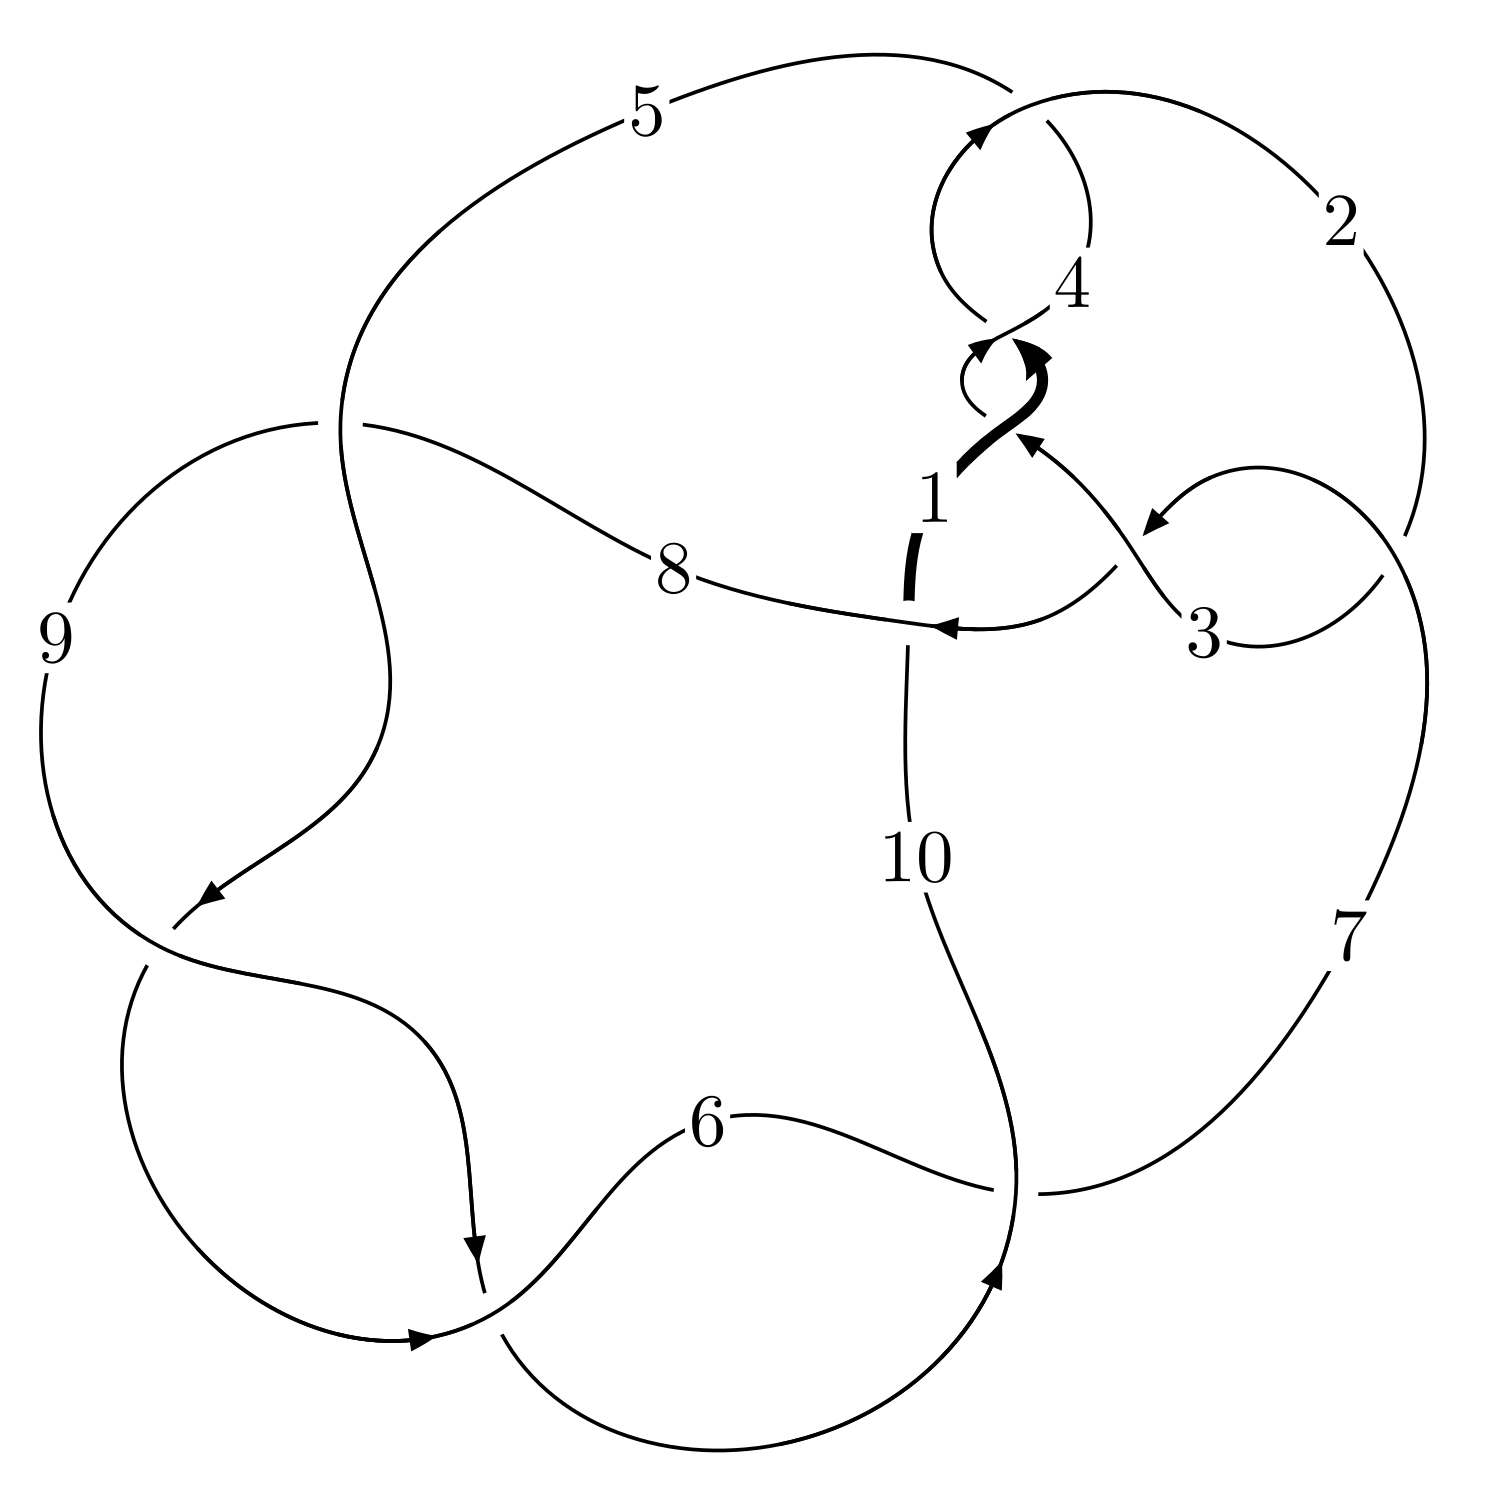
\includegraphics[width=112pt]{../../../GIT/diagram.site/Diagrams/png/132_10_48.png}\\
\ \ \ A knot diagram\footnotemark}&
\allowdisplaybreaks
\textbf{Linearized knot diagam} \\
\cline{2-2}
 &
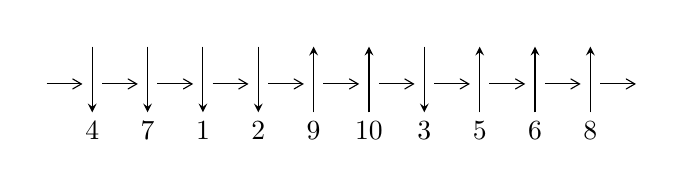
\begin{tikzpicture}[x=20pt, y=17pt]
	% nodes
	\node (C0) at (0, 0) {};
	\node (C1) at (1, 0) {};
	\node (C1U) at (1, +1) {};
	\node (C1D) at (1, -1) {4};

	\node (C2) at (2, 0) {};
	\node (C2U) at (2, +1) {};
	\node (C2D) at (2, -1) {7};

	\node (C3) at (3, 0) {};
	\node (C3U) at (3, +1) {};
	\node (C3D) at (3, -1) {1};

	\node (C4) at (4, 0) {};
	\node (C4U) at (4, +1) {};
	\node (C4D) at (4, -1) {2};

	\node (C5) at (5, 0) {};
	\node (C5U) at (5, +1) {};
	\node (C5D) at (5, -1) {9};

	\node (C6) at (6, 0) {};
	\node (C6U) at (6, +1) {};
	\node (C6D) at (6, -1) {10};

	\node (C7) at (7, 0) {};
	\node (C7U) at (7, +1) {};
	\node (C7D) at (7, -1) {3};

	\node (C8) at (8, 0) {};
	\node (C8U) at (8, +1) {};
	\node (C8D) at (8, -1) {5};

	\node (C9) at (9, 0) {};
	\node (C9U) at (9, +1) {};
	\node (C9D) at (9, -1) {6};

	\node (C10) at (10, 0) {};
	\node (C10U) at (10, +1) {};
	\node (C10D) at (10, -1) {8};
	\node (C11) at (11, 0) {};

	% arrows
	\draw[->,>={angle 60}]
	(C0) edge (C1) (C1) edge (C2) (C2) edge (C3) (C3) edge (C4) (C4) edge (C5) (C5) edge (C6) (C6) edge (C7) (C7) edge (C8) (C8) edge (C9) (C9) edge (C10) (C10) edge (C11) ;	\draw[->,>=stealth]
	(C1U) edge (C1D) (C2U) edge (C2D) (C3U) edge (C3D) (C4U) edge (C4D) (C5D) edge (C5U) (C6D) edge (C6U) (C7U) edge (C7D) (C8D) edge (C8U) (C9D) edge (C9U) (C10D) edge (C10U) ;
	\end{tikzpicture} \\
\hhline{~~} \\& 
\textbf{Solving Sequence} \\ \cline{2-2} 
 &
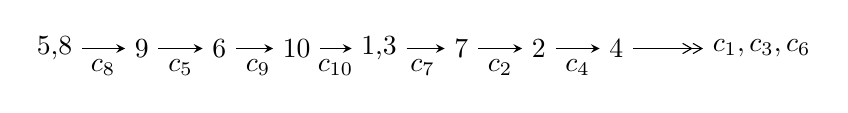
\begin{tikzpicture}[x=28pt, y=7pt]
	% node
	\node (A0) at (-1/8, 0) {5,8};
	\node (A1) at (1, 0) {9};
	\node (A2) at (2, 0) {6};
	\node (A3) at (3, 0) {10};
	\node (A4) at (65/16, 0) {1,3};
	\node (A5) at (41/8, 0) {7};
	\node (A6) at (49/8, 0) {2};
	\node (A7) at (57/8, 0) {4};
	\node (C1) at (1/2, -1) {$c_{8}$};
	\node (C2) at (3/2, -1) {$c_{5}$};
	\node (C3) at (5/2, -1) {$c_{9}$};
	\node (C4) at (7/2, -1) {$c_{10}$};
	\node (C5) at (37/8, -1) {$c_{7}$};
	\node (C6) at (45/8, -1) {$c_{2}$};
	\node (C7) at (53/8, -1) {$c_{4}$};
	\node (A8) at (9, 0) {$c_{1},c_{3},c_{6}$};

	% edge
	\draw[->,>=stealth]	
	(A0) edge (A1) (A1) edge (A2) (A2) edge (A3) (A3) edge (A4) (A4) edge (A5) (A5) edge (A6) (A6) edge (A7) ;
	\draw[->>,>={angle 60}]	
	(A7) edge (A8);
\end{tikzpicture} \\ 

\end{tabular} \\

\footnotetext{
The image of knot diagram is generated by the software ``\textbf{Draw programme}" developed by Andrew Bartholomew(\url{http://www.layer8.co.uk/maths/draw/index.htm\#Running-draw}), where we modified some parts for our purpose(\url{https://github.com/CATsTAILs/LinksPainter}).
}\phantom \\ \newline 
\centering \textbf{Ideals for irreducible components\footnotemark of $X_{\text{par}}$} 
 
\begin{align*}
I^u_{1}&=\langle 
u^{25}-14 u^{23}+\cdots+b-1,\;- u^{24}+u^{23}+\cdots+a+2,\;u^{26}-2 u^{25}+\cdots+3 u+1\rangle \\
I^u_{2}&=\langle 
b,\;a- u-1,\;u^2+u-1\rangle \\
\\
\end{align*}
\raggedright * 2 irreducible components of $\dim_{\mathbb{C}}=0$, with total 28 representations.\\
\footnotetext{All coefficients of polynomials are rational numbers. But the coefficients are sometimes approximated in decimal forms when there is not enough margin.}
\newpage
\renewcommand{\arraystretch}{1}
\centering \section*{I. $I^u_{1}= \langle u^{25}-14 u^{23}+\cdots+b-1,\;- u^{24}+u^{23}+\cdots+a+2,\;u^{26}-2 u^{25}+\cdots+3 u+1 \rangle$}
\flushleft \textbf{(i) Arc colorings}\\
\begin{tabular}{m{7pt} m{180pt} m{7pt} m{180pt} }
\flushright $a_{5}=$&$\begin{pmatrix}0\\u\end{pmatrix}$ \\
\flushright $a_{8}=$&$\begin{pmatrix}1\\0\end{pmatrix}$ \\
\flushright $a_{9}=$&$\begin{pmatrix}1\\- u^2\end{pmatrix}$ \\
\flushright $a_{6}=$&$\begin{pmatrix}u\\- u^3+u\end{pmatrix}$ \\
\flushright $a_{10}=$&$\begin{pmatrix}- u^2+1\\u^4-2 u^2\end{pmatrix}$ \\
\flushright $a_{1}=$&$\begin{pmatrix}u^4-3 u^2+1\\u^4-2 u^2\end{pmatrix}$ \\
\flushright $a_{3}=$&$\begin{pmatrix}u^{24}- u^{23}+\cdots+4 u-2\\- u^{25}+14 u^{23}+\cdots+5 u+1\end{pmatrix}$ \\
\flushright $a_{7}=$&$\begin{pmatrix}- u^3+2 u\\u^5-3 u^3+u\end{pmatrix}$ \\
\flushright $a_{2}=$&$\begin{pmatrix}u^{24}- u^{23}+\cdots+u-3\\u^{25}-14 u^{23}+\cdots-2 u-1\end{pmatrix}$ \\
\flushright $a_{4}=$&$\begin{pmatrix}u^{24}- u^{23}+\cdots+2 u-2\\u^{14}-8 u^{12}+\cdots- u^2+2 u\end{pmatrix}$\\&\end{tabular}
\flushleft \textbf{(ii) Obstruction class $= -1$}\\~\\
\flushleft \textbf{(iii) Cusp Shapes $= 3 u^{24}- u^{23}-41 u^{22}+8 u^{21}+237 u^{20}-2 u^{19}-754 u^{18}-180 u^{17}+1435 u^{16}+802 u^{15}-1634 u^{14}-1608 u^{13}+954 u^{12}+1718 u^{11}+24 u^{10}-1034 u^9-412 u^8+379 u^7+265 u^6-70 u^5-147 u^4+10 u^3+32 u^2+18 u-7$}\\~\\
\newpage\renewcommand{\arraystretch}{1}
\flushleft \textbf{(iv) u-Polynomials at the component}\newline \\
\begin{tabular}{m{50pt}|m{274pt}}
Crossings & \hspace{64pt}u-Polynomials at each crossing \\
\hline $$\begin{aligned}c_{1},c_{3},c_{4}\end{aligned}$$&$\begin{aligned}
&u^{26}-3 u^{25}+\cdots-9 u^2-1
\end{aligned}$\\
\hline $$\begin{aligned}c_{2},c_{7}\end{aligned}$$&$\begin{aligned}
&u^{26}- u^{25}+\cdots+17 u^2-4
\end{aligned}$\\
\hline $$\begin{aligned}c_{5},c_{6},c_{8}\\c_{9}\end{aligned}$$&$\begin{aligned}
&u^{26}-2 u^{25}+\cdots+3 u+1
\end{aligned}$\\
\hline $$\begin{aligned}c_{10}\end{aligned}$$&$\begin{aligned}
&u^{26}+6 u^{25}+\cdots+57 u-9
\end{aligned}$\\
\hline
\end{tabular}\\~\\
\newpage\renewcommand{\arraystretch}{1}
\flushleft \textbf{(v) Riley Polynomials at the component}\newline \\
\begin{tabular}{m{50pt}|m{274pt}}
Crossings & \hspace{64pt}Riley Polynomials at each crossing \\
\hline $$\begin{aligned}c_{1},c_{3},c_{4}\end{aligned}$$&$\begin{aligned}
&y^{26}-25 y^{25}+\cdots+18 y+1
\end{aligned}$\\
\hline $$\begin{aligned}c_{2},c_{7}\end{aligned}$$&$\begin{aligned}
&y^{26}-15 y^{25}+\cdots-136 y+16
\end{aligned}$\\
\hline $$\begin{aligned}c_{5},c_{6},c_{8}\\c_{9}\end{aligned}$$&$\begin{aligned}
&y^{26}-30 y^{25}+\cdots-19 y+1
\end{aligned}$\\
\hline $$\begin{aligned}c_{10}\end{aligned}$$&$\begin{aligned}
&y^{26}+6 y^{25}+\cdots-3159 y+81
\end{aligned}$\\
\hline
\end{tabular}\\~\\
\newpage\flushleft \textbf{(vi) Complex Volumes and Cusp Shapes}
$$\begin{array}{c|c|c}  
\text{Solutions to }I^u_{1}& \I (\text{vol} + \sqrt{-1}CS) & \text{Cusp shape}\\
 \hline 
\begin{aligned}
u &= -0.668864 + 0.598628 I \\
a &= -1.61808 + 1.14418 I \\
b &= -1.31336 - 0.55274 I\end{aligned}
 & -6.97144 - 7.45946 I & -3.34661 + 6.43325 I \\ \hline\begin{aligned}
u &= -0.668864 - 0.598628 I \\
a &= -1.61808 - 1.14418 I \\
b &= -1.31336 + 0.55274 I\end{aligned}
 & -6.97144 + 7.45946 I & -3.34661 - 6.43325 I \\ \hline\begin{aligned}
u &= \phantom{-}1.198900 + 0.140779 I \\
a &= -0.217750 - 0.235577 I \\
b &= -1.276500 - 0.100979 I\end{aligned}
 & -3.39138 - 0.04941 I & -2.26185 - 0.23755 I \\ \hline\begin{aligned}
u &= \phantom{-}1.198900 - 0.140779 I \\
a &= -0.217750 + 0.235577 I \\
b &= -1.276500 + 0.100979 I\end{aligned}
 & -3.39138 + 0.04941 I & -2.26185 + 0.23755 I \\ \hline\begin{aligned}
u &= -0.586941 + 0.484436 I \\
a &= \phantom{-}1.86292 - 1.18885 I \\
b &= \phantom{-}1.051360 + 0.358584 I\end{aligned}
 & -0.89453 - 3.84444 I & -0.49259 + 7.28090 I \\ \hline\begin{aligned}
u &= -0.586941 - 0.484436 I \\
a &= \phantom{-}1.86292 + 1.18885 I \\
b &= \phantom{-}1.051360 - 0.358584 I\end{aligned}
 & -0.89453 + 3.84444 I & -0.49259 - 7.28090 I \\ \hline\begin{aligned}
u &= -0.283620 + 0.683381 I \\
a &= \phantom{-}1.65331 - 0.64793 I \\
b &= \phantom{-}1.330650 - 0.398492 I\end{aligned}
 & -8.11148 + 3.15061 I & -5.88075 - 0.93673 I \\ \hline\begin{aligned}
u &= -0.283620 - 0.683381 I \\
a &= \phantom{-}1.65331 + 0.64793 I \\
b &= \phantom{-}1.330650 + 0.398492 I\end{aligned}
 & -8.11148 - 3.15061 I & -5.88075 + 0.93673 I \\ \hline\begin{aligned}
u &= \phantom{-}0.486887 + 0.485193 I \\
a &= \phantom{-}0.722742 - 0.089263 I \\
b &= -0.151101 - 1.041920 I\end{aligned}
 & -3.27468 + 1.70414 I & -2.66466 - 3.89699 I \\ \hline\begin{aligned}
u &= \phantom{-}0.486887 - 0.485193 I \\
a &= \phantom{-}0.722742 + 0.089263 I \\
b &= -0.151101 + 1.041920 I\end{aligned}
 & -3.27468 - 1.70414 I & -2.66466 + 3.89699 I\\
 \hline 
 \end{array}$$\newpage$$\begin{array}{c|c|c}  
\text{Solutions to }I^u_{1}& \I (\text{vol} + \sqrt{-1}CS) & \text{Cusp shape}\\
 \hline 
\begin{aligned}
u &= \phantom{-}0.622264 + 0.175930 I \\
a &= -0.280102 - 0.073287 I \\
b &= \phantom{-}0.338732 + 0.457385 I\end{aligned}
 & \phantom{-}1.166700 + 0.399409 I & \phantom{-}7.28789 - 1.42640 I \\ \hline\begin{aligned}
u &= \phantom{-}0.622264 - 0.175930 I \\
a &= -0.280102 + 0.073287 I \\
b &= \phantom{-}0.338732 - 0.457385 I\end{aligned}
 & \phantom{-}1.166700 - 0.399409 I & \phantom{-}7.28789 + 1.42640 I \\ \hline\begin{aligned}
u &= -0.345528 + 0.459270 I \\
a &= -2.06279 + 0.67901 I \\
b &= -0.939749 + 0.103171 I\end{aligned}
 & -1.59551 + 0.48344 I & -4.02832 + 0.08458 I \\ \hline\begin{aligned}
u &= -0.345528 - 0.459270 I \\
a &= -2.06279 - 0.67901 I \\
b &= -0.939749 - 0.103171 I\end{aligned}
 & -1.59551 - 0.48344 I & -4.02832 - 0.08458 I \\ \hline\begin{aligned}
u &= \phantom{-}1.51750 + 0.08533 I \\
a &= \phantom{-}1.165270 + 0.679850 I \\
b &= \phantom{-}1.069430 - 0.265042 I\end{aligned}
 & \phantom{-}4.66926 + 1.10360 I & \phantom{-}0.162083 - 0.384354 I \\ \hline\begin{aligned}
u &= \phantom{-}1.51750 - 0.08533 I \\
a &= \phantom{-}1.165270 - 0.679850 I \\
b &= \phantom{-}1.069430 + 0.265042 I\end{aligned}
 & \phantom{-}4.66926 - 1.10360 I & \phantom{-}0.162083 + 0.384354 I \\ \hline\begin{aligned}
u &= -1.53355 + 0.12553 I \\
a &= -0.351346 + 0.586908 I \\
b &= \phantom{-}0.393229 - 1.143620 I\end{aligned}
 & \phantom{-}3.48759 - 3.82064 I & \phantom{-}0.89607 + 2.40126 I \\ \hline\begin{aligned}
u &= -1.53355 - 0.12553 I \\
a &= -0.351346 - 0.586908 I \\
b &= \phantom{-}0.393229 + 1.143620 I\end{aligned}
 & \phantom{-}3.48759 + 3.82064 I & \phantom{-}0.89607 - 2.40126 I \\ \hline\begin{aligned}
u &= \phantom{-}1.56506 + 0.13930 I \\
a &= -0.92214 - 1.07989 I \\
b &= -1.134790 + 0.523946 I\end{aligned}
 & \phantom{-}6.35171 + 6.10679 I & \phantom{-}2.97747 - 5.14405 I \\ \hline\begin{aligned}
u &= \phantom{-}1.56506 - 0.13930 I \\
a &= -0.92214 + 1.07989 I \\
b &= -1.134790 - 0.523946 I\end{aligned}
 & \phantom{-}6.35171 - 6.10679 I & \phantom{-}2.97747 + 5.14405 I\\
 \hline 
 \end{array}$$\newpage$$\begin{array}{c|c|c}  
\text{Solutions to }I^u_{1}& \I (\text{vol} + \sqrt{-1}CS) & \text{Cusp shape}\\
 \hline 
\begin{aligned}
u &= -1.58442 + 0.05231 I \\
a &= \phantom{-}0.214222 - 0.374662 I \\
b &= -0.346659 + 0.743600 I\end{aligned}
 & \phantom{-}8.75625 - 1.27302 I & \phantom{-}7.34031 + 0.88258 I \\ \hline\begin{aligned}
u &= -1.58442 - 0.05231 I \\
a &= \phantom{-}0.214222 + 0.374662 I \\
b &= -0.346659 - 0.743600 I\end{aligned}
 & \phantom{-}8.75625 + 1.27302 I & \phantom{-}7.34031 - 0.88258 I \\ \hline\begin{aligned}
u &= \phantom{-}1.59031 + 0.18503 I \\
a &= \phantom{-}0.687931 + 1.166390 I \\
b &= \phantom{-}1.28311 - 0.68193 I\end{aligned}
 & \phantom{-}0.59945 + 10.37890 I & -0.23306 - 5.66856 I \\ \hline\begin{aligned}
u &= \phantom{-}1.59031 - 0.18503 I \\
a &= \phantom{-}0.687931 - 1.166390 I \\
b &= \phantom{-}1.28311 + 0.68193 I\end{aligned}
 & \phantom{-}0.59945 - 10.37890 I & -0.23306 + 5.66856 I \\ \hline\begin{aligned}
u &= -1.67318\phantom{ +0.000000I} \\
a &= -0.394205\phantom{ +0.000000I} \\
b &= \phantom{-}0.856853\phantom{ +0.000000I}\end{aligned}
 & \phantom{-}6.22196\phantom{ +0.000000I} & -3.01540\phantom{ +0.000000I} \\ \hline\begin{aligned}
u &= -0.282820\phantom{ +0.000000I} \\
a &= -3.31419\phantom{ +0.000000I} \\
b &= -0.465579\phantom{ +0.000000I}\end{aligned}
 & -1.22611\phantom{ +0.000000I} & -10.4970\phantom{ +0.000000I}\\
 \hline 
 \end{array}$$\newpage\newpage\renewcommand{\arraystretch}{1}
\centering \section*{II. $I^u_{2}= \langle b,\;a- u-1,\;u^2+u-1 \rangle$}
\flushleft \textbf{(i) Arc colorings}\\
\begin{tabular}{m{7pt} m{180pt} m{7pt} m{180pt} }
\flushright $a_{5}=$&$\begin{pmatrix}0\\u\end{pmatrix}$ \\
\flushright $a_{8}=$&$\begin{pmatrix}1\\0\end{pmatrix}$ \\
\flushright $a_{9}=$&$\begin{pmatrix}1\\u-1\end{pmatrix}$ \\
\flushright $a_{6}=$&$\begin{pmatrix}u\\- u+1\end{pmatrix}$ \\
\flushright $a_{10}=$&$\begin{pmatrix}u\\- u\end{pmatrix}$ \\
\flushright $a_{1}=$&$\begin{pmatrix}0\\- u\end{pmatrix}$ \\
\flushright $a_{3}=$&$\begin{pmatrix}u+1\\0\end{pmatrix}$ \\
\flushright $a_{7}=$&$\begin{pmatrix}1\\0\end{pmatrix}$ \\
\flushright $a_{2}=$&$\begin{pmatrix}u+1\\0\end{pmatrix}$ \\
\flushright $a_{4}=$&$\begin{pmatrix}u+1\\u\end{pmatrix}$\\&\end{tabular}
\flushleft \textbf{(ii) Obstruction class $= 1$}\\~\\
\flushleft \textbf{(iii) Cusp Shapes $= 5$}\\~\\
\newpage\renewcommand{\arraystretch}{1}
\flushleft \textbf{(iv) u-Polynomials at the component}\newline \\
\begin{tabular}{m{50pt}|m{274pt}}
Crossings & \hspace{64pt}u-Polynomials at each crossing \\
\hline $$\begin{aligned}c_{1}\end{aligned}$$&$\begin{aligned}
&(u-1)^2
\end{aligned}$\\
\hline $$\begin{aligned}c_{2},c_{7}\end{aligned}$$&$\begin{aligned}
&u^2
\end{aligned}$\\
\hline $$\begin{aligned}c_{3},c_{4}\end{aligned}$$&$\begin{aligned}
&(u+1)^2
\end{aligned}$\\
\hline $$\begin{aligned}c_{5},c_{6}\end{aligned}$$&$\begin{aligned}
&u^2- u-1
\end{aligned}$\\
\hline $$\begin{aligned}c_{8},c_{9},c_{10}\end{aligned}$$&$\begin{aligned}
&u^2+u-1
\end{aligned}$\\
\hline
\end{tabular}\\~\\
\newpage\renewcommand{\arraystretch}{1}
\flushleft \textbf{(v) Riley Polynomials at the component}\newline \\
\begin{tabular}{m{50pt}|m{274pt}}
Crossings & \hspace{64pt}Riley Polynomials at each crossing \\
\hline $$\begin{aligned}c_{1},c_{3},c_{4}\end{aligned}$$&$\begin{aligned}
&(y-1)^2
\end{aligned}$\\
\hline $$\begin{aligned}c_{2},c_{7}\end{aligned}$$&$\begin{aligned}
&y^2
\end{aligned}$\\
\hline $$\begin{aligned}c_{5},c_{6},c_{8}\\c_{9},c_{10}\end{aligned}$$&$\begin{aligned}
&y^2-3 y+1
\end{aligned}$\\
\hline
\end{tabular}\\~\\
\newpage\flushleft \textbf{(vi) Complex Volumes and Cusp Shapes}
$$\begin{array}{c|c|c}  
\text{Solutions to }I^u_{2}& \I (\text{vol} + \sqrt{-1}CS) & \text{Cusp shape}\\
 \hline 
\begin{aligned}
u &= \phantom{-}0.618034\phantom{ +0.000000I} \\
a &= \phantom{-}1.61803\phantom{ +0.000000I} \\
b &= \phantom{-0.000000 } 0\end{aligned}
 & -0.657974\phantom{ +0.000000I} & \phantom{-}5.00000\phantom{ +0.000000I} \\ \hline\begin{aligned}
u &= -1.61803\phantom{ +0.000000I} \\
a &= -0.618034\phantom{ +0.000000I} \\
b &= \phantom{-0.000000 } 0\end{aligned}
 & \phantom{-}7.23771\phantom{ +0.000000I} & \phantom{-}5.00000\phantom{ +0.000000I}\\
 \hline 
 \end{array}$$\newpage
\newpage\renewcommand{\arraystretch}{1}
\centering \section*{ III. u-Polynomials}
\begin{tabular}{m{50pt}|m{274pt}}
Crossings & \hspace{64pt}u-Polynomials at each crossing \\
\hline $$\begin{aligned}c_{1}\end{aligned}$$&$\begin{aligned}
&((u-1)^2)(u^{26}-3 u^{25}+\cdots-9 u^2-1)
\end{aligned}$\\
\hline $$\begin{aligned}c_{2},c_{7}\end{aligned}$$&$\begin{aligned}
&u^2(u^{26}- u^{25}+\cdots+17 u^2-4)
\end{aligned}$\\
\hline $$\begin{aligned}c_{3},c_{4}\end{aligned}$$&$\begin{aligned}
&((u+1)^2)(u^{26}-3 u^{25}+\cdots-9 u^2-1)
\end{aligned}$\\
\hline $$\begin{aligned}c_{5},c_{6}\end{aligned}$$&$\begin{aligned}
&(u^2- u-1)(u^{26}-2 u^{25}+\cdots+3 u+1)
\end{aligned}$\\
\hline $$\begin{aligned}c_{8},c_{9}\end{aligned}$$&$\begin{aligned}
&(u^2+u-1)(u^{26}-2 u^{25}+\cdots+3 u+1)
\end{aligned}$\\
\hline $$\begin{aligned}c_{10}\end{aligned}$$&$\begin{aligned}
&(u^2+u-1)(u^{26}+6 u^{25}+\cdots+57 u-9)
\end{aligned}$\\
\hline
\end{tabular}\newpage\renewcommand{\arraystretch}{1}
\centering \section*{ IV. Riley Polynomials}
\begin{tabular}{m{50pt}|m{274pt}}
Crossings & \hspace{64pt}Riley Polynomials at each crossing \\
\hline $$\begin{aligned}c_{1},c_{3},c_{4}\end{aligned}$$&$\begin{aligned}
&((y-1)^2)(y^{26}-25 y^{25}+\cdots+18 y+1)
\end{aligned}$\\
\hline $$\begin{aligned}c_{2},c_{7}\end{aligned}$$&$\begin{aligned}
&y^2(y^{26}-15 y^{25}+\cdots-136 y+16)
\end{aligned}$\\
\hline $$\begin{aligned}c_{5},c_{6},c_{8}\\c_{9}\end{aligned}$$&$\begin{aligned}
&(y^2-3 y+1)(y^{26}-30 y^{25}+\cdots-19 y+1)
\end{aligned}$\\
\hline $$\begin{aligned}c_{10}\end{aligned}$$&$\begin{aligned}
&(y^2-3 y+1)(y^{26}+6 y^{25}+\cdots-3159 y+81)
\end{aligned}$\\
\hline
\end{tabular}
\vskip 2pc
\end{document}